% Template for Cogsci submission with R Markdown

% Stuff changed from original Markdown PLOS Template
\documentclass[10pt, letterpaper]{article}

\usepackage{cogsci}
\usepackage{pslatex}
\usepackage{float}

% amsmath package, useful for mathematical formulas
\usepackage{amsmath}

% amssymb package, useful for mathematical symbols
\usepackage{amssymb}

% hyperref package, useful for hyperlinks
\usepackage{hyperref}

% graphicx package, useful for including eps and pdf graphics
% include graphics with the command \includegraphics
\usepackage{graphicx}

% Sweave(-like)
\usepackage{fancyvrb}
\DefineVerbatimEnvironment{Sinput}{Verbatim}{fontshape=sl}
\DefineVerbatimEnvironment{Soutput}{Verbatim}{}
\DefineVerbatimEnvironment{Scode}{Verbatim}{fontshape=sl}
\newenvironment{Schunk}{}{}
\DefineVerbatimEnvironment{Code}{Verbatim}{}
\DefineVerbatimEnvironment{CodeInput}{Verbatim}{fontshape=sl}
\DefineVerbatimEnvironment{CodeOutput}{Verbatim}{}
\newenvironment{CodeChunk}{}{}

% cite package, to clean up citations in the main text. Do not remove.
\usepackage{cite}

\usepackage{color}

% Use doublespacing - comment out for single spacing
%\usepackage{setspace}
%\doublespacing


% % Text layout
% \topmargin 0.0cm
% \oddsidemargin 0.5cm
% \evensidemargin 0.5cm
% \textwidth 16cm
% \textheight 21cm

\title{Determining the alternatives for scalar implicature}


\author{{\large \bf Benjamin Peloquin} \\ \texttt{bpeloqui@stanford.edu} \\ Department of Psychology \\ Stanford University \And {\large \bf Michael C. Frank} \\ \texttt{mcfrank@stanford.edu} \\ Department of Psychology \\ Stanford University}

\begin{document}

\maketitle

\begin{abstract}
Successful communication regularly requires listeners to make pragmatic
inferences - enrichments beyond the literal meaning of a speaker's
utterance. For example, when interpreting a sentence such as ``Alice ate
some of the cookies,'' listeners routinely infer that Alice did not eat
all of them. A Gricean account of this phenomena assumes the presence of
alternatives (like ``all of the cookies'') with varying degrees of
informativity, but it remains an open question precisely what these
alternatives are. To address this question, we collect empirical
measurements of speaker and listener judgments about varying sets of
alternatives across a range of scales and use these as inputs to a
computational model of pragmatic inference. This approach allows us to
test hypotheses about how well different sets of alternatives predict
pragmatic judgments by people. Our findings suggest that comprehenders
likely consider a broader set of alternatives beyond those logically
entailed by the initial message.

\textbf{Keywords:}
pragmatics; scalar implicature; bayesian modeling
\end{abstract}

\section{Introduction}\label{introduction}

How much of what we mean comes from the words that go unsaid? As
listeners, our ability to make precise inferences about a speaker's
intended meaning in context is indispensable to successful
communication. For example, listeners commonly enrich the meaning of the
scalar item \emph{some} to \emph{some but not all} in sentences like
``Alice ate some of the cookies'' (Grice, 1975; Levinson, 2000). These
inferences, called \emph{scalar implicatures}, have been an important
test case for understanding pragmatic inferences more generally. A
Gricean account of this phenomenon assumes listeners reason about a
speaker's intended meaning by incorporating knowledge about A)
alternative scalar items a speaker could have used (such as \emph{all})
and B) the relative informativity of using such alternatives (Grice,
1975). According to this account, a listener will infer that the speaker
must have intended that Alice did not eat all the cookies because it
would have been underinformative to use the descriptor \emph{some} when
the alternative \emph{all} could have been used just as easily.

But what are the alternatives that should be considered in the
implicature computation more generally? Under classic accounts,
listeners consider only those words whose meanings entail the actual
message (Horn, 1972), and these alternatives enter into conventionalized
or semi-conventionalized scales (Levinson, 2000). For example, because
\emph{all} entails \emph{some}, and hence is a ``stronger'' meaning,
\emph{all} should be considered as an alternative to \emph{some} in
implicatures. Similar scales exist for non-quantifier scales, e.g.
\emph{loved} entails \emph{liked} (and hence ``I liked the movie''
implicates that I didn't love it).

Recent empirical evidence has called into question whether entailment
scales are all that is necessary for understanding scalar implicature.
For example, Degen \& Tanenhaus (2015) demonstrated that the scalar item
\emph{some} was judged less appropriate when exact numbers were seen as
viable alternatives. And in a different paradigm, {van Tiel} (2014)
found converging evidence that \emph{some} was judged to be atypical for
small quantities. These data provide indirect evidence that people may
actually consider a broader set of alternatives when computing scalar
implicatures. Since \emph{some} is logically true of sets with one or
two members, these authors argued that the presence of salient
alternatives (the words \emph{one} and \emph{two}, for example) reduced
the felicity of \emph{some} via a pragmatic inference.

By formalizing pragmatic reasoning, computational models can help
provide more direct evidence about the role that alternatives play. The
``rational speech act'' model (RSA) is one recent framework for
understanding inferences about meaning in context (Frank \& Goodman,
2012; Goodman \& Stuhlmuller, 2013). RSA models frame language
understanding as a special case of social cognition, in which listeners
and speakers reason recursively about one another's goals. In the case
of scalar implicature, a listener makes a probabilistic inference about
what the speaker's most likely communicative goal was, given that she
picked the quantifier \emph{some} rather than the stronger quantifier
\emph{all}. In turn, the speaker reasons about what message would best
convey her intended meaning to the listener, given that he is reasoning
in this way. This recursion is grounded in a ``literal'' listener who
reasons only according to the basic truth-functional semantics of the
language.

Franke (2014) used an RSA-style model to assess what alternatives a
speaker would need to consider in order to produce the
typicality/felicity ratings reported by Degen \& Tanenhaus (2015) and
{van Tiel} (2014) for the scale \emph{some}/\emph{all}. In order to do
this, Franke (2014)'s model assigned weights to a set of alternative
numerical expressions. Surprisingly, along with weighting \emph{one}
highly (a conclusion that was supported by the empirical work), the
best-fitting model assigned substantial weight to \emph{none} as an
alternative to \emph{some}. This finding was especially surprising
considering the emphasis of standard theories on scalar items that stand
in entailment relationships with one another (e.g. \emph{one} entails
\emph{some} even if it is not classically considered to be part of the
scale).

In our current work, we pick up where these previous studies left off,
considering the set of alternatives for implicature using the RSA model.
To gain empirical traction on this issue, however, we broaden the set of
scales we consider. Our inspiration for this move comes from work by
{van Tiel}, Van Miltenburg, Zevakhina, \& Geurts (2014), who examined a
phenomenon that they dubbed ``scalar diversity,'' namely the substantial
difference in the strength of scalar implicature across a variety of
scalar pairs (e.g., \emph{liked} / \emph{loved,} \emph{palatable} /
\emph{delicious}). Making use of this diversity allows us to investigate
the ways that different alternative sets give rise to implicatures of
different strengths across scales.

In our current work, we use a computational framework to investigate the
set of alternatives that best allow the model to predict human pragmatic
judgments. We begin by presenting the computational framework (RSA) we
use throughout the paper. We next describe a series of experiments
designed to measure both the literal semantics of a set of scalar items
(used to simulate different alternative sets available to listeners) and
comprehenders' pragmatic judgments for these same items (used for model
comparison). These experiments allow us to compare the effects of
different alternative sets on our ability to model listeners' pragmatic
judgments. To preview our results: we find that standard entailment
alternatives do not allow us to fit participants' judgments, but that
expanding the range of alternatives empirically (by asking participants
to generate alternative messages) allows us to predict listeners'
pragmatic judgments with high accuracy.

\section{Modeling Implicature Using
RSA}\label{modeling-implicature-using-rsa}

We begin by giving a brief presentation of the basic RSA model. This
model simulates the judgments of a pragmatic listener who wants to infer
a speaker's intended meaning \(m\) from her utterance \(u\). For
simplicity, we present a version of this model in which there is only
one full recursion: The pragmatic listener reasons about a pragmatic
speaker, who in turn reasons about a ``literal listener.'' We assume
throughout that this computation takes place in a signaling game (Lewis,
1969) with a fixed set of possible meanings \(m \in M\) and a fixed
possible set of utterances \(u \in U\), with both known to both
participants. Our goal in this study is to determine which utterances
fall in \(U\).

In the standard RSA model, the pragmatic listener (denoted \(L_1\)),
makes a Bayesian inference:

\[p_{L_1}(m \mid u) \propto p_{S_1} (u \mid m) p(m) \tag{1}\]

\noindent In other words, the probability of a particular meaning given
an utterance is proportional to the speaker's probability of using that
particular utterance to express that meaning, weighted by a prior over
meanings. This prior represents the listener's \emph{a priori}
expectations about plausible meanings, independent of the utterance.
Because our experiments take place in a context in which listeners
should have very little expectation about which meanings speakers want
to convey, for simplicity we assume a uniform prior where
\(p(m) \propto 1\).

The pragmatic speaker in turn considers the probability that a literal
listener would interpret her utterance correctly:

\[p_{S_1}(u \mid m) \propto p_{L_0} (m \mid u) \tag{2}\]

\noindent where \(L_0\) refers to a listener who only considers the
truth-functional semantics of the utterance (that is, which meanings the
utterance can refer to).

This model of the pragmatic speaker (denoted \(S_1\)) is consistent with
a speaker who chooses words to maximize the utility of an utterance in
context (Frank \& Goodman, 2012), where utility is operationalized as
the informativity of a particular utterance (surprisal) minus a cost:

\[p_{S_1}(u \mid m) \propto e^{-\alpha[-log(p_{L_0}(m \mid u)) - C(u)]} \tag{3}\]

\noindent where \(C(u)\) is the cost of a particular utterance,
\(-log(p_{L_0})\) represents the \emph{surprisal} of the message for the
literal listener (the information content of the utterance), and
\(\alpha\) is a parameter in a standard choice rule. If \(\alpha=0\),
speakers choose randomly; as \(\alpha \rightarrow \infty\), they
greedily choose the highest probability alternative. In our simulations
below, we treat \(\alpha\) as a free parameter and fit it to the data.

To instantiate our signaling game with a tractable message set \(M\), in
our studies we adopt the world of restaurant reviews as our
communication game. We assume that speakers and listeners are trying to
communicate the number of stars in an online restaurant review (where
\(m \in \{1...5\}\)). We then use experiments to measure three
components of the model. First, to generate a set of plausible
alternative messages in \(U\), we ask participants to generate
alternatives for particular scalar items (Experiment 1). Next, to
measure literal semantics \({p_{L_0} (m \mid u)}\) we ask participants
to judge whether a message is compatible with a particular meaning
(Experiment 2). Lastly, to obtain human \(L_1\) pragmatic judgments, we
ask participants to interpret a speaker's utterances (Experiment 3).

\begin{CodeChunk}
\begin{figure}[t]
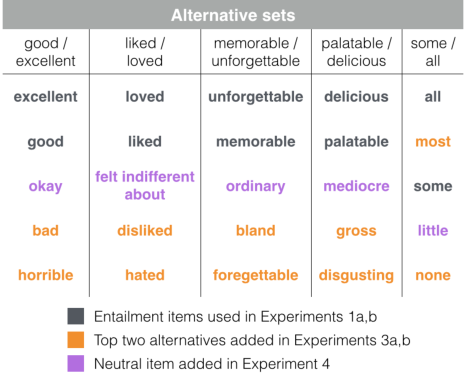
\includegraphics{figs/allScalesTable-1} \caption[Alternative sets used in Experiments 2 and 3]{Alternative sets used in Experiments 2 and 3. Green coloring denotes classic entailment items used in conditions 2a and 3a. Blue coloring denotes top-two alternatives added to entailment scales (from Experiment 1) in conditions 2b and 3b. Red coloring denotes ``neutral" items aded in condition 2c.}\label{fig:allScalesTable}
\end{figure}
\end{CodeChunk}

\begin{CodeChunk}
\begin{figure}[t]

{\centering 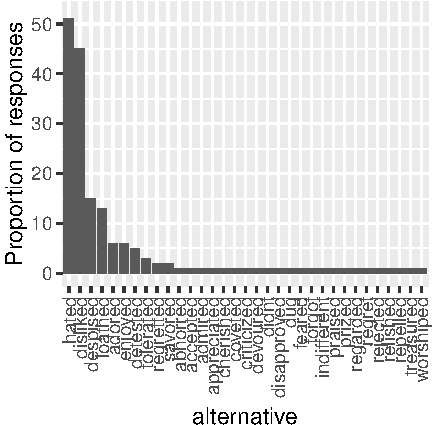
\includegraphics{figs/exp2_altsPlot_likedLoved-1} 

}

\caption[Combined counts for participant-generated alternatives for liked vs]{Combined counts for participant-generated alternatives for liked vs. loved in Experiment 2.}\label{fig:exp2_altsPlot_likedLoved}
\end{figure}
\end{CodeChunk}

\section{Experiment 1: Alternative
Elicitation}\label{experiment-1-alternative-elicitation}

To examine the effect different alternative sets have on implicature, we
needed a way of expanding alternative sets beyond entailment pairs. We
addressed this issue by adopting a modified cloze task to elicit
alternatives empirically. This design was inspired by Experiment 3 of
{van Tiel} (2014).

\subsection{Methods}\label{methods}

\subsubsection{Participants}\label{participants}

We recruited 30 workers on AMT. All participants were native English
speakers and naive to the purpose of the experiment.

\subsubsection{Design and procedure}\label{design-and-procedure}

Participants were presented with a target scalar item from five scales,
selected from {van Tiel} et al. (2014) (see Figure
\ref{fig:allScalesTable}). These were embedded in a sentence such as,
``In a recent restaurant review someone said they thought the the food
was \_\_\_\_," with a target scalar presented in the blank. Participants
were then asked to generate plausible alternatives by responding to the
question, ``If they'd felt differently about the food, what other words
could they have used instead of \_\_\_\_?" They were prompted to
generate three unique alternatives.

\subsection{Results and Discussion}\label{results-and-discussion}

\begin{CodeChunk}
\begin{figure*}[t]

{\centering 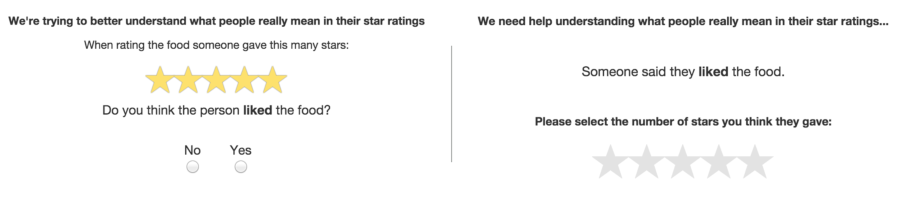
\includegraphics{figs/stimuli_exp1-1} 

}

\caption[(Left) A trial from Experiment 2 (literal listener) with the target scalar "liked]{(Left) A trial from Experiment 2 (literal listener) with the target scalar "liked."(Right) A trial from Experiment 3 (pragmatic listener) with the target scalar "liked."}\label{fig:stimuli_exp1}
\end{figure*}
\end{CodeChunk}

Figure \ref{fig:exp2_altsPlot_likedLoved} shows an example alternative
set for the scalar items \emph{liked} and \emph{loved} (combined).
Figure \ref{fig:allScalesTable} shows the complete list of alternative
sets derived from Experiment 1.

\section{Experiment 2: Literal listener
task}\label{experiment-2-literal-listener-task}

Experiment 2 was conducted to approximate literal listener
semantics---\(p_{L_0}(m \mid u)\) in Equation (3)---for the same five
pairs of scalar items used in Experiment 1. We included three
conditions: two alternatives (``entailment''), four alternatives, and
five alternatives. The two alternatives condition makes a test of the
hypothesis that the two members of the classic Horn (entailment) scale
(Horn, 1972) are the only alternatives necessary to predict the strength
of listeners' pragmatic inference. The four and five alternatives
conditions then add successively more alternatives to test whether
including a larger number of alternatives will increase model
fit.\footnote{Note that alternatives in the four and five alternatives conditions were chosen on the basis of Experiment 1, which was run chronologically after the two-alternative condition; all literal listener experiments are grouped together for simplicity in reporting.}
A secondary goal of Experiment 2 is to test whether the set of
alternatives queried during literal semantic elicitation impacts literal
semantic judgments. If it does we should see differences in these
judgments for shared items between experiments.

\subsection{Methods}\label{methods-1}

\subsubsection{Participants}\label{participants-1}

Conditions were run sequentially. In each condition we recruited 30
participants from Amazon Mechanical Turk (AMT). In the two alternatives
condition, 16 participants were excluded for either failing to pass two
training trials or because they were not native English speakers,
leaving a total sample of 14
participants.\footnote{The majority of respondent data excluded from the two-alternatives condition was caused by failure to pass training trials. We believe the task may have been too difficult for most respondents and made adjustments to the training trials in later conditions.}
In the four alternative condition, 7 participants were excluded for
either failing to pass two training trials or not being native English
speakers, leaving a total sample of 23 participants. In the five
alternative condition, 3 participants were excluded for either failing
to pass two training trials or not being native English speakers,
leaving a total sample of 27.

\subsubsection{Design and procedure}\label{design-and-procedure-1}

Figure \ref{fig:stimuli_exp1}, left, shows the experimental setup.
Participants were presented with a target scalar item and a star rating
(1--5 stars) and asked to judge the compatibility of the scalar item and
star rating. Compatibility was assessed through a binary ``yes/no''
response to a question of the form, ``Do you think that the person
thought the food was \_\_\_\_?" where a target scalar was presented in
the blank. Each participant saw all scalar item and star rating
combinations for their particular condition, in a random order.

The two-alternatives condition included only the two terms in the pairs
from van Tiel (2014). The four-alternatives condition included the two
scalar items plus the top two alternatives generated for each scalar
family by participants in Experiment 1. The five-alternatives condition
included the four previous items plus one more neutral item chosen from
alternatives generated in Experiment 1.

\subsection{Results and Discussion}\label{results-and-discussion-1}

\begin{CodeChunk}
\begin{figure*}[t]

{\centering 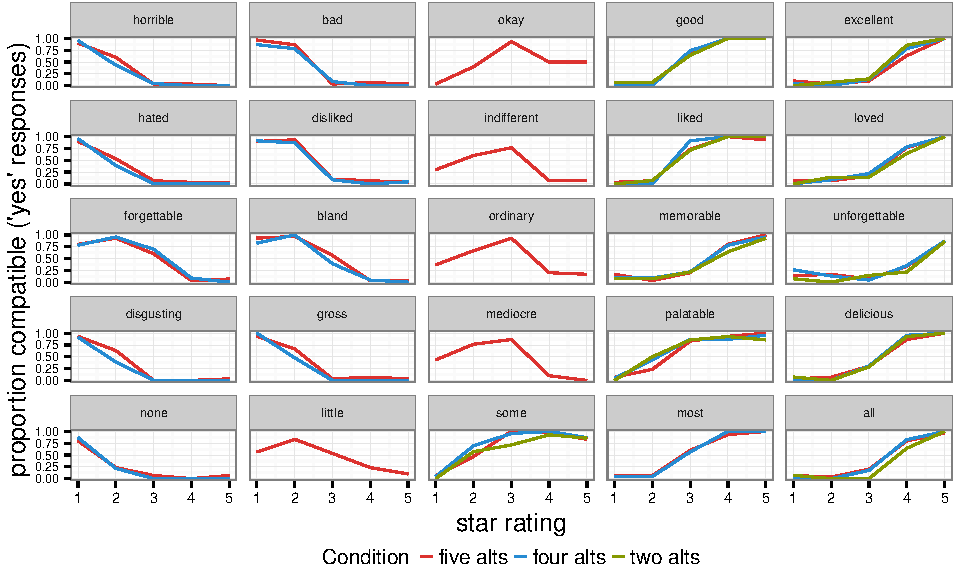
\includegraphics{figs/exp1Plots-1} 

}

\caption[Literal listener judgments from Experiment 2]{Literal listener judgments from Experiment 2. Proportion of participants indicating compatibility (answering "yes") is shown on the vertical axis, with the horizontal axis showing number of stars on which the utterance was judged. Rows are grouped by scale and items within rows are ordered by valence. Colors indicate the specific condition (1a,b,c) with conditions including different numbers of items.}\label{fig:exp1Plots}
\end{figure*}
\end{CodeChunk}

Figure \ref{fig:exp1Plots} plots estimated literal listener semantics
for the three conditions. Each row shows a unique scalar family with
items ordered horizontally by valence. Several trends are visible.
First, in each scale, the alternatives spanned the star scale - there
were scalar items that were highly compatible with both the lowest and
highest numbers of stars. Second, participant compatibility judgments
match intuitive literal semantics. That is, both weaker (e.g.
\emph{some} or \emph{good}) and stronger (e.g. \emph{all} or
\emph{excellent}) entailment items were seen as compatible with
five-star ratings. This means participants' compatibility judgements
reflect literal semantic intuitions, not enriched pragmatic judgments.
We see clear variability between scalar families (literal semantic
distributions for \emph{memorable} are considerably different from
\emph{palatable}), but also substantial consistency across conditions
(compatibility judgments for individual items are consistent across
conditions).

To examine this last issue of consistency across conditions (our
secondary hypothesis) we fit a mixed effects model, regressing
compatibility judgment on scale, number of stars and experimental
condition, with subject- and word-level random effects, which was the
maximal structure that converged. Results indicate no significant
differences between two- and five-alternative conditions
(\(\beta=-0.05\), \(z = -0.53\), \(p = 0.59\)) or between four- and
five-alternative conditions (\(\beta = -0.04\), \(z = -0.52\),
\(p = 0.6\)). The addition of condition as a predictor did not
significantly improve model fit when compared to a model without the
condition variable using ANOVA (\(\chi^2(2) = 0.43\), \(p = 0.81\)).
These findings suggest that literal semantic intuitions are not affected
by the set of alternatives queried in our paradigm. This finding is
important because literal semantic data generated in these three
conditions are used to simulate the effects of different alternative
sets on implicature generation in our model.

\section{Experiment 3: Pragmatic
Listener}\label{experiment-3-pragmatic-listener}

Experiment 3 was conducted to measure pragmatic judgments. As in
Experiment 2, we include several conditions to test inferences in the
presence of different alternative sets. In the two alternatives
condition, participants made judgments for items included in the
entailment scales. In the four alternatives condition, participants made
judgments for the entailment items and also the top two alternatives
elicited for each scale in Experiment 1. Including two conditions with
differing alternatives allowed us to rule out the potential effects of
having a larger set of alternatives during the pragmatic judgment
elicitation and also provided two sets of human judgments to compare
with model predictions.

\subsection{Participants}\label{participants-2}

We recruited 100 participants from AMT, 50 for each condition. Data for
9 participants was excluded from the two alternatives condition after
participants either failed to pass two training trials or were
non-native English speakers, leaving a total sample of 41 participants.
In the four alternatives condition, data from 7 participants was
excluded after participants either failed to pass two training trials or
were not native English speakers, leaving 43 participants.

\subsection{Procedure}\label{procedure}

Participants were presented with a one-sentence prompt such as ``Someone
said they thought the food was \_\_\_\_\_.'' with a target scalar item
in the blank. Participants were then asked to generate a star rating
representing the rating they thought the reviewer likely gave. Each
participant was presented with all scalar items in a random order. The
experimental setup is shown in Figure \ref{fig:stimuli_exp1}, right.

\subsection{Results and Discussion}\label{results-and-discussion-2}

\begin{CodeChunk}
\begin{figure*}[t]

{\centering 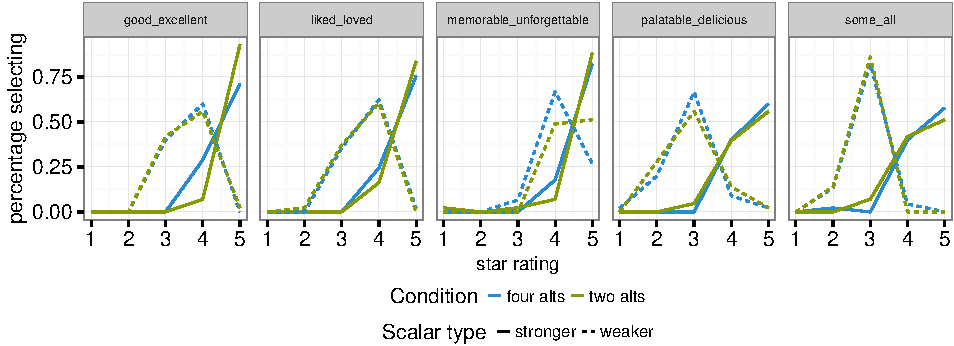
\includegraphics{figs/exp2Plots-1} 

}

\caption[Pragmatic listener judgements in Experiment 3]{Pragmatic listener judgements in Experiment 3. Proportion of participants generating a star rating is shown on the vertical axis, with the horizontal axis showing number of stars on which the utterance was judged. Line type denotes condition, and colors indicate the particular scalar items. Each panel shows one scalar pair, with only entailment items (two alternatives condition) shown here for simplicity in reporting.}\label{fig:exp2Plots}
\end{figure*}
\end{CodeChunk}

Figure \ref{fig:exp2Plots} plots pragmatic listener judgment
distributions for ``weak'' / ``strong'' scalar pairs (e.g.
\emph{good}/\emph{excellent}). Several trends are visible. First, in
each scale participants generated implicatures. They were substantially
less likely to assign high star ratings to weaker scalar terms, despite
the literal semantic compatibility of those terms with those states
shown in Experiment 2. Second, the difference between strong and weak
scalar items varied considerably across scales, consistent with previous
work ({van Tiel} et al., 2014).

To rule out the potential effects of having a larger set of alternatives
during the pragmatic judgment elicitation, we fit a mixed effects model.
We regressed pragmatic judgments on scale and experimental condition
with subject- and word-level random effects, which was the maximal
structure that converged. There were no significant differences between
the two alternatives and four alternatives conditions (\(\beta = 0.05\),
\(t(150) = 1.04\), \(p = 0.3\)). The addition of the condition predictor
did not significantly improve model fit when compared to a model without
that variable (\(\chi^2(1) = 1.13\), \(p = 0.29\)).

\section{Model}\label{model}

Using literal listener data from Experiment 2, we conducted a set of
simulations with the RSA model. Each simulation kept the model constant,
fitting the choice parameter \(\alpha\) as a free parameter, but used a
set of alternatives to specify the scale over which predictions were
computed. We considered four different alternative sets, with empirical
measurements corresponding to those shown in Figure
\ref{fig:allScalesTable}: 1) the two alternatives in the classic
entailment scales, 2) those two alternatives with the addition of a
generic negative alternative, 3) the expanded set of four alternatives,
and 4) the expanded set of five alternatives. Literal semantics for the
generic negative alternative serve as a baseline ``none``-style
semantics in which the scalar item is only compatible with 1 star.

Model fit with human judgments was significantly improved by the
inclusion of alternatives beyond the entailment items (Table 1). The
two-alternatives model contained only entailment items, which, under
classic accounts, should be sufficient to generate implicature, but fit
to data was quite poor with these items. The addition of a generic
negative element produced some gains in performance, but much higher
performance was found when we included four and five alternatives, with
the alternatives derived empirically for the specific scale we used. An
example fit for the five-alternatives model is shown in Figure
\ref{fig:fiveAltsScatter}.

\begin{table}[ht]
\centering
\begin{tabular}{lrrr}
  \hline
Model & $\alpha$ & Two alts & Four alts \\ 
  \hline
Two alts &   9 & 0.54 & 0.57 \\ 
  Two alts + generic negative  &   6 & 0.62 & 0.66 \\ 
  Four alts &   4 & 0.84 & 0.90 \\ 
  Five alts &   4 & 0.86 & 0.90 \\ 
   \hline
\end{tabular}
\caption{Model performance with fitted alpha levels. Model fit assessed through correlation with human judgments in the two conditions of Experiment 3.} 
\end{table}

\section{General Discussion}\label{general-discussion}

Pragmatic inference requires reasoning about alternatives. The
fundamental pragmatic computation is counterfactual: ``if she had meant
X, she would have said Y, but she didn't.'' Yet the nature of these
alternatives has been controversial. For a few well-studied scales, a
small set of logically-determined alternatives has been claimed to be
all that is necessary (Horn, 1972). For other, contextually-determined
inferences, the issue of alternatives has been considered relatively
intractable in terms of formal inquiry (Sperber \& Wilson, 1995).

In our current work, we used the rational speech act framework to
investigate the set of alternatives that best allowed the model to
predict pragmatic judgments across a series of different scales. We
found that the best predictions came when a range of scale-dependent
negative and neutral alternatives were added to the implicature
computation, suggesting the importance of considering non-entailment
alternatives. This work builds on previous investigations, reinforcing
the claim that negative alternatives are critical for understanding
implicature (Franke, 2014), and replicates and extends findings that
different lexical scales produce strikingly different patterns of
inference ({van Tiel} et al., 2014).

While improvements in model fit were substantial as we moved from two to
four alternatives, we saw only a minor increase in fit from the move to
five alternatives. One possible explanation is that alternatives are
differentially salient in context, and in moving to larger sets we
should consider weighting the alternatives differentially (as Franke,
2014 did). Preliminary simulations using weightings derived from
Experiment 1 provide some support for this idea but would require
further empirical work for confirmation.

The precise set of alternatives present during implicature is likely to
be domain dependent. Our empirical paradigm elicited literal semantics,
pragmatic judgments, and plausible alternatives all within the
restricted domain of restaurant reviews. Our measurements might have
differed substantially if we had instead grounded our ratings in a
different context. Future investigations should probe the
context-specificity of the weight and availability of particular
alternative sets.

More broadly, considering the context- and domain-specificity of
alternative sets may provide a way to unite what Grice (1975) called
``generalized'' (cross-context) and ``particularized''
(context-dependent) implicatures. Rather than being grounded in a firm
distinction, we may find that these categories are simply a reflection
of the effects of context on a constantly-shifting set of pragmatic
alternatives.

\begin{CodeChunk}
\begin{figure}[t]
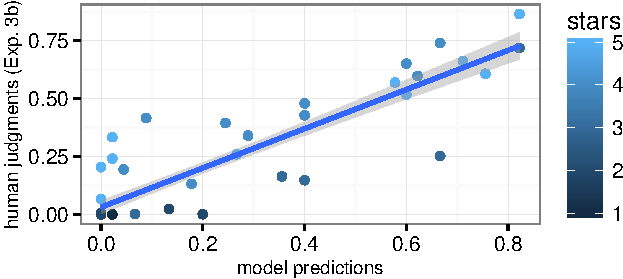
\includegraphics{figs/fiveAltsScatter-1} \caption[Judgments from the four-alternatives condition of Experiment 3 are plotted against model predictions using the five-alternatives data from Experiment 1]{Judgments from the four-alternatives condition of Experiment 3 are plotted against model predictions using the five-alternatives data from Experiment 1. Colors show the star rating for individual judgments.}\label{fig:fiveAltsScatter}
\end{figure}
\end{CodeChunk}

\section{Acknowledgements}\label{acknowledgements}

Thanks to NSF BCS \#1456077 for support, and thanks to Michael Franke,
Judith Degen, and Noah Goodman for valuable discussion.

\section{References}\label{references}

\setlength{\parindent}{-0.1in} \setlength{\leftskip}{0.125in} \noindent

Degen, J., \& Tanenhaus, M. K. (2015). Processing scalar implicature: A
constraint-based approach. \emph{Cognitive Science}, \emph{39}(4),
667--710.

Frank, M., \& Goodman, N. D. (2012). Predicting pragmatic reasoning in
language games. \emph{Science}, \emph{336}(6084), 998.

Franke, M. (2014). Typical use of quantifiers: A probabilistic speaker
model. In \emph{Proceedings of the 36th annual conference of the
cognitive science society} (pp. 487--492).

Goodman, N. D., \& Stuhlmuller, A. (2013). Knowledge and implicature:
Modeling language understanding as social cognition. \emph{Topics in
Cognitive Science}, \emph{5}(1), 173--184.

Grice, H. P. (1975). Logic and conversation. In P. Cole \& J. Morgan
(Eds.), \emph{Syntax and semantics} (Vol. 3). New York: Academic Press.

Horn, L. R. (1972). \emph{On the semantic properties of logical
operators.} (PhD thesis). University of California, Los Angeles.

Levinson, S. C. (2000). \emph{Presumptive meanings: The theory of
generalized conversational implicature}. MIT Press.

Lewis, D. (1969). \emph{Convention: A philosophical study}. John Wiley
\& Sons.

Sperber, D., \& Wilson, D. (1995). \emph{Relevance: Communication and
cognition} (2nd ed.). Oxford, UK: Blackwell.

{van Tiel}, B. J. M. (2014). Quantity matters: Implicatures, typicality,
and truth.

{van Tiel}, B. J. M., Van Miltenburg, E., Zevakhina, N., \& Geurts, B.
(2014). Scalar diversity. \emph{Journal of Semantics}, ffu017.

\end{document}
